\documentclass[a4paper,12pt]{article}
\usepackage{amsmath,amsthm,amsfonts,amssymb,amscd,amstext,vmargin,graphics,graphicx,tabularx,multicol} 
\usepackage[francais]{babel}
\usepackage[utf8]{inputenc}  
\usepackage[T1]{fontenc} 
\usepackage{pstricks-add,tikz,tkz-tab,variations}
\usepackage[autolanguage,np]{numprint} 

\setmarginsrb{2cm}{1cm}{2cm}{0.5cm}{0cm}{0cm}{0cm}{0cm} %Gauche, haut, droite, haut
\newcounter{numexo}
\newcommand{\exo}[1]{\stepcounter{numexo}\noindent{\bf Exercice~\thenumexo} : \marginpar{\hfill /#1}}
\reversemarginpar


\newcounter{enumtabi}
\newcounter{enumtaba}
\newcommand{\q}{\textbf{\stepcounter{enumtabi} \theenumtabi)}  }
\newcommand{\qa}{\textbf{\stepcounter{enumtaba} (\alph{enumtaba})} }
\newcommand{\initq}{\setcounter{enumtabi}{0}}
\newcommand{\initqa}{\setcounter{enumtaba}{0}}

\newcommand{\be}{\begin{enumerate}}
\newcommand{\ee}{\end{enumerate}}
\newcommand{\bi}{\begin{itemize}}
\newcommand{\ei}{\end{itemize}}
\newcommand{\bp}{\begin{pspicture*}}
\newcommand{\ep}{\end{pspicture*}}
\newcommand{\bt}{\begin{tabular}}
\newcommand{\et}{\end{tabular}}
\renewcommand{\tabularxcolumn}[1]{>{\centering}m{#1}} %(colonne m{} centrée, au lieu de p par défault) 
\newcommand{\tnl}{\tabularnewline}

\newcommand{\bmul}[1]{\begin{multicols}{#1}}
\newcommand{\emul}{\end{multicols}}

\newcommand{\trait}{\noindent \rule{\linewidth}{0.2mm}}
\newcommand{\hs}[1]{\hspace{#1}}
\newcommand{\vs}[1]{\vspace{#1}}

\newcommand{\N}{\mathbb{N}}
\newcommand{\Z}{\mathbb{Z}}
\newcommand{\R}{\mathbb{R}}
\newcommand{\C}{\mathbb{C}}
\newcommand{\Dcal}{\mathcal{D}}
\newcommand{\Ccal}{\mathcal{C}}
\newcommand{\mc}{\mathcal}

\newcommand{\vect}[1]{\overrightarrow{#1}}
\newcommand{\ds}{\displaystyle}
\newcommand{\eq}{\quad \Leftrightarrow \quad}
\newcommand{\vecti}{\vec{\imath}}
\newcommand{\vectj}{\vec{\jmath}}
\newcommand{\Oij}{(O;\vec{\imath}, \vec{\jmath})}
\newcommand{\OIJ}{(O;I,J)}


\newcommand{\reponse}[1][1]{%
\multido{}{#1}{\makebox[\linewidth]{\rule[0pt]{0pt}{20pt}\dotfill}
}}

\newcommand{\titre}[5] 
% #1: titre #2: haut gauche #3: bas gauche #4: haut droite #5: bas droite
{
\noindent #2 \hfill #4 \\
#3 \hfill #5

\vspace{-1.6cm}

\begin{center}\rule{6cm}{0.5mm}\end{center}
\vspace{0.2cm}
\begin{center}{\large{\textbf{#1}}}\end{center}
\begin{center}\rule{6cm}{0.5mm}\end{center}
}



\begin{document}
\pagestyle{empty}
\titre{Correction contrôle 2 : Fonctions affines }{Nom :}{Prénom :}{\textbf{2nd 8}}{Date:}



\exo{5.5} Les fonctions suivantes sont-elles affines ? Si oui ,donner leurs coefficients directeurs et leurs ordonnées à l'origine.\\

\initqa \qa $f(x)=-9x+6$ \qa $g(x)=3x^2+5$ \qa $h(x)=-2(4-3x)$\\

 \qa $j(x)=\dfrac{10}{3x}$ \qa $f(x)=\dfrac{x-2}{9}$\\

\color{purple}

\initqa \qa La fonction $f$ est une fonction affine avec m = -9 et p = 6.\\
\qa La fonction $g$ n'est pas une fonction affine car $x$ est au carré.\\
\qa $h(x)=-8+6x$ donc la fonction $h$ est une fonction affine avec m = 6 et p = -8.\\
\qa La fonction $j$ n'est pas une fonction affine car $x$ est au dénominateur.\\
\qa $f(x)=\dfrac{x}{9}-\dfrac{2}{9}$ donc la fonction $f$ est une fonction affine avec $m=\dfrac{1}{9}$  et $p=-\dfrac{2}{9}$.\\


\color{black}
\vspace*{0.5cm}

\exo{4.5}On munit le plan d’un repère orthogonal.\\
Sur le graphique ci-contre, on a représenté deux fonctions $f$ et $g$ sur l'intervalle [-10;14].\\
On note $D_f$  et $D_g$ les droites qui représentent respectivement les fonctions affines $f$ et $g$.\\
\includegraphics[scale=1.5]{lecturegraphique.eps} \\

 \initq \q Quelle est l'image de -2 par la fonction $f$ ? \textcolor{purple}{L'image de -2 par la fonction $f$ est 6.}\\

\q Quelle est l'image de 8 par la fonction $g$ ? \textcolor{purple}{L'image de 8 par la fonction $g$ est 8.}\\

\q Déterminer $f(10)$? \textcolor{purple}{f(10)= 0.}\\

\q Lire le ou les antécédent(s) de 8 par la fonction $f$ ?\textcolor{purple}{L'antécédent de 8 par la fonction $f$ est -6.}\\

\q Lire le ou les antécédent(s) de 2  par la fonction $g$ ?\textcolor{purple}{L'antécédent de 2 par la fonction $g$ est -1.}\\

\q Quelle est l'abscisse du point de $C_f$ d'ordonnée 5 ?\textcolor{purple}{L'abscisse  du point de $C_f$ d'ordonnée 5  est 0.}\\

\q Quel est l'ensemble des solutions de l'équation $g(x)=-4$ ?\textcolor{purple}{Cela revient à chercher l'antécédent de -4 par $g$, l'ensemble solution est $S=\lbrace -10\rbrace$.}\\

\q Quel est l'ensemble des solutions de l'équation $f(x)>0$ ?\textcolor{purple}{Cela revient à chercher tous les $x$ pour lesquels la fonction $f$ est strictement positive, l'ensemble solution est $S=[-10;10[$.}\\


\vspace*{0.5cm}

\exo{6} Soient $f$ et $g$ deux fonctions affines définies par $f(x)=-3x+20$ et  $g(x)=\dfrac{5-3x}{10}$.\\

 \initq \q Calculer l'image de -3 par la fonction $f$ .\\
 
 \color{purple}
 $f(-3)=-3 \times (-3)+20$\\
  $f(-3)=9+20$\\
 \fbox{$f(-3)=29$}\\
  \color{black}

\q Calculer l'image de 0 par la fonction $g$ .\\

\color{purple}
 $g(0)=\dfrac{5-3\times 0}{10}$\\
  $g(0)=\dfrac{5}{10}$\\
 \fbox{$g(0)=0,5$}\\
  \color{black}

\q  Calculer $f\left(\dfrac{4}{3}\right)$.\\

\color{purple}
 $f\left(\dfrac{4}{3}\right)=-3 \times \dfrac{4}{3} +20$\\
 $f\left(\dfrac{4}{3}\right)=-\dfrac{12}{3} +\dfrac{60}{3}$\\
 \fbox{$f\left(\dfrac{4}{3}\right)=\dfrac{48}{3}=16 $}\\
  \color{black}

\q Déterminer les antécédents éventuels de 18,5 par f .\\

 \color{purple}
Pour cela, nous allons résoudre l'équation suivante  $f(x)=18,5$.\\
Soit, $-3x+20=18,5$ $\Leftrightarrow$ $-3x=-1,5$ $\Leftrightarrow$ \fbox{$x=0,5$}\\
  \color{black}

\q Quelle est l'abscisse du point de $C_f$ d'ordonnée 0 ?\\

\color{purple}
Pour cela, nous allons résoudre l'équation suivante  $f(x)=0$.\\
Soit, $-3x+20=0$ $\Leftrightarrow$ $-3x=-20$ $\Leftrightarrow$ \fbox{$x=\dfrac{20}{3}$}\\
  \color{black}

\newpage


\exo{4} Pour les trois droites représentées ci-dessous, déterminer
leurs coefficients directeurs, leurs ordonnées à l'origine puis les expressions des fonctions affines correspondant aux droites.

\bmul{2}


\includegraphics[scale=1.3]{representation2.eps} 

\columnbreak

\color{purple}
Cherchons les coefficients $m$ et $p$ pour chacune des fonctions affines.\\

\bi
\item La fonction g est une fonction constante avec m = 0 et p = 8. Donc $g(x)=8$\\
\item La fonction $f$ est une fonction affine avec m = 4 et p = 1. Donc $f(x)=4x+1$\\
\item La fonction $h$ est une fonction affine avec m = -2 et p = 4. Donc $h(x)=-2x+4$\\
\item La fonction $j$ est une fonction affine avec $m=-\dfrac{3}{2}=-1,5$ et p = -2. Donc $j(x)=-1,5x-2$\\
\ei

  \color{black}


\emul



\vspace*{0.5cm}


\exo{} \textbf{BONUS} \\
\textbf{Reprenons l'exercice 2.} D'abord graphiquement puis par le calcul, déterminer l'ensemble des solutions de l'équation $f(x)=g(x)$?\\

\end{document}
